\subsection{Komplexe Zahlen 2}
\Aufgabe{
    Es gelte für folgende komplexe Zahlen: \\
    $K_1 = 10 + j40$  \\
    $K_2 = 50 \cdot e^{-j40^o}$   \\
    $K_3 = 250 \cdot e^{j\frac{\pi}{4}}$    \\
    
    Berechnet werden sollen folgende Aufgabenteile:
    \begin{itemize}
        \item [\bf a)] $K_1 - K_2$, Ergebnis in Polarkoordinaten
        \item [\bf b)] $K_3 + K_2$, Ergebnis in kartesischen Koordinaten
        \item [\bf c)] $K_1 \cdot K_3$, Ergebnis in Polarkoordinaten
        \item [\bf d)] $K_1 + K_2$, zeichnerisch im Zeigerdiagramm
        \item [\bf e)] $(K_1 - K_2)^2$
        \item [\bf f)] $\sqrt{K_1 + K_3}$
    \end{itemize}
}


\Loesung{
    \begin{itemize}

        \item[\bf a)]   $K_1 - K_2$, Ergebnis in Polarkoordinaten
              
              \begin{eqa}
                  10 + \mathrm{j} \cdot 40 - 50 \cdot \mathrm{e}^{-\mathrm{j}40^\circ} = ? \nonumber 
              \end{eqa}
              
              $\underline{K}_2$ in kartesische Koordinaten wandeln: 
              
              \begin{eqa}
                  50 \cdot \mathrm{e}^{-\mathrm{j}40^\circ} &= 50 \cdot \cos(-40^\circ) + \mathrm{j} 50 \cdot \sin(-40^\circ)  \nonumber   \\
                  &= 50 \cdot 0,766 + \mathrm{j} 50 \cdot (-0,6427)  \nonumber   \\
                  &= 38,302 - \mathrm{j} 32,1393  \nonumber
              \end{eqa}
              
              $\underline{K}_2 - \underline{K}_2$ in kartesischen Koordinaten subtrahieren: 
              
              \begin{eqa}
                  \underline{K}_1 - \underline{K}_2 &= (10 + \mathrm{j} \cdot 40) - (38,302 - \mathrm{j} 32,1393) \nonumber   \\
                  &= 10 + \mathrm{j} \cdot 40 - 38,302 + \mathrm{j} 32,1393 \nonumber   \\
                  &= -28,3 + \mathrm{j} 72,139    \nonumber
              \end{eqa}
              
              Ergebnis in Polarkoordinaten: 
              
              \begin{eqa}
                  \underline{K}_1 - \underline{K}_2 &= \sqrt{\Re^2+\Im^2} \cdot \mathrm{e}^{\mathrm{j}\arctan(\frac{\Im}{\Re})} \nonumber   \\
                  &= 77,49 \cdot \mathrm{e}^{\mathrm{j}111,42^\circ}  \nonumber
              \end{eqa}
              
        \item[\bf b)] $K_3 + K_2$, Ergebnis in kartesischen Koordinaten
              
              \begin{eqa}
                  K_3 &= 250 \cdot e^{j\frac{\pi}{4}} = 176,78 + j176,78  \nonumber   \\
                  K_2 &= 50 \cdot e^{-j40^\circ} = 38,3 - j32,15  \nonumber   \\
                  K_3 + K_2 &= (176,78 + j176,78) + (38,3 - j32,15)  \nonumber   \\
                  K_3 + K_2 &= 215,08 + j144,63  \nonumber   
              \end{eqa}
              
        \item[\bf c)] $K_1 \cdot K_3$, Ergebnis in Polarkoordinaten
              
              \begin{eqa}
                  \underline{K}_1 &= 10 + \mathrm{j}40   \nonumber   \\
                  &= 41,23 \cdot \mathrm{e}^{\mathrm{j}75,96^\circ}  \nonumber  \\
                  \underline{K}_1 \cdot \underline{K}_3 &= 10 + \mathrm{j}40  \cdot 250 \cdot \mathrm{e}^{\mathrm{j}45^\circ}    \nonumber   \\
                  &= 10307,75 \cdot \mathrm{e}^{\mathrm{j}120,96^\circ}  \nonumber  
              \end{eqa}
              
        \item[\bf d)] $K_1 + K_2$, zeichnerisch im Zeigerdiagramm
              
              \begin{figure}[H]
                  \centering
                  \resizebox{0.3\textwidth}{!}{
                      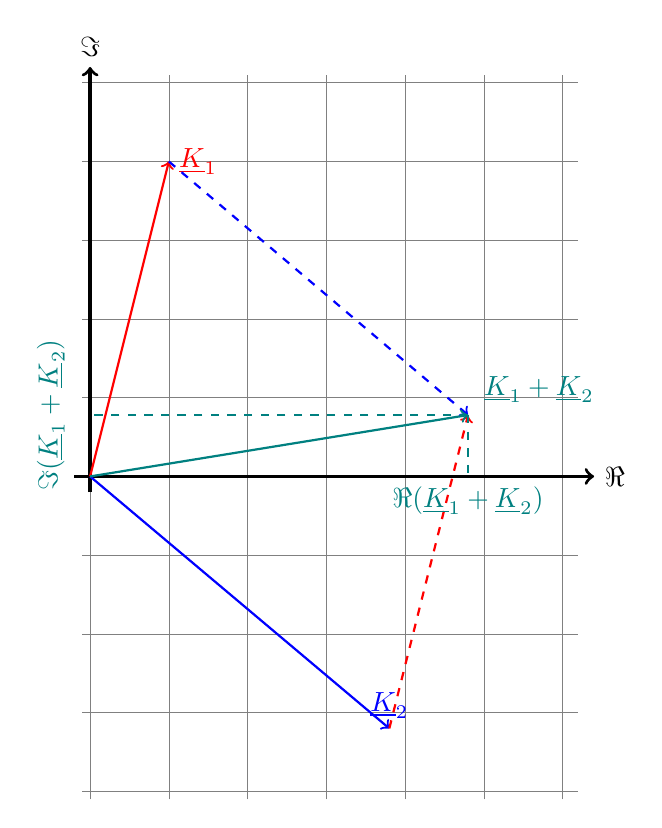
\begin{tikzpicture}
    \draw (0,0) coordinate (K);
    \draw[very thin,gray] (-0.1,-4.1) grid (6.2,5.1);
    \draw[->, very thick] (-0.2,0) -- (6.4,0) node[right] {$\Re$};
    \draw[->, very thick] (0,-0.2) -- (0,5.2) node[above] {$\Im$};
    \draw[->, thick, red] (0,0) -- (1,4) node[right] {$\underline{K}_\mathrm{1}$};
    \draw[->, thick, blue] (0,0) -- (3.8,-3.2) node[above] {$\underline{K}_\mathrm{2}$};

    \draw[->, dashed, thick, blue] (1,4) -- (4.8,0.78);
    \draw[->, dashed, thick, red] (3.8,-3.2) -- (4.8,0.78);


    \draw[->, thick, teal] (0,0) -- (4.8,0.78);
    \draw(5.7,1.1) node [teal] {$\underline{K}_\mathrm{1}+\underline{K}_\mathrm{2}$};
    \draw[dashed, thick, teal] (4.8,0.78) -- (0,0.78)
    (-0.5,0.78) node[rotate=90] {$\Im(\underline{K}_\mathrm{1}+\underline{K}_\mathrm{2}$)};
    \draw[dashed, thick, teal] (4.8,0.78) -- (4.8,0) node[below] {$\Re(\underline{K}_\mathrm{1}+\underline{K}_\mathrm{2}$)};
\end{tikzpicture}
                  }
              \end{figure}
              
        \item[\bf e)] $(K_1 - K_2)^2$
              
              Ergebnis aus Teil a): 
              \begin{eqa}
                  K_1 - Z_2 = 77,49 \cdot \mathrm{e}^{\mathrm{j}111,42^\circ} \nonumber  
              \end{eqa}
              
              Regel für das Quadrat einer komplexen Zahl:
              \begin{eqa}
                  (K_1 - K_2)^2 &= 77,49^2 \cdot \mathrm{e}^{\mathrm{j}2 \cdot 111,42^\circ}    \nonumber   \\
                  &= 6004 \cdot \mathrm{e}^{-\mathrm{j}137^\circ} \nonumber 
              \end{eqa}
              
              
        \item[\bf f)] $\sqrt{K_1 + K_3}$
              
              \begin{eqa}
                  K_1 + K_3 = 186,78 + j216,78    \nonumber   
              \end{eqa}
              
              Umwandlung in Polarform:
              
              \begin{eqa}
                  K_1 + K_3 = 286,09 \cdot \mathrm{e}^{\mathrm{j}49,32^\circ}   \nonumber   
              \end{eqa}
              
              Die Quadratwurzel einer komplexen Zahl in Polarform ergibt:
              
              \begin{eqa}
                  \sqrt{r \cdot \mathrm{e}^{\mathrm{j}\varphi}} &= \sqrt{r} \frac{\varphi}{2}  \nonumber   \\
                  \sqrt{286,09} \cdot \mathrm{e}^{\mathrm{j}\frac{49,32^\circ}{2}} &= 16,91 \cdot \mathrm{e}^{\mathrm{j}24,66^\circ}  \nonumber
              \end{eqa}
              
    \end{itemize}
    
}